\documentclass{article}
\usepackage{amsmath}
\usepackage{amsfonts}
\usepackage[inline]{enumitem}
\usepackage[a4paper,margin=1in]{geometry}
\usepackage{fancyhdr}
\setlength{\headheight}{36pt}
\usepackage[normalem]{ulem}
\usepackage{graphicx}
\fancyhf{}
\renewcommand{\headrulewidth}{0pt}

\begin{document}

\thispagestyle{fancy}
\lhead{Calculus Exercise}
\chead{Week 1 (1.4, 1.5, 2.1)}
\rhead{\underline{ID:\hspace{7.4em}} \\ \vspace{0.2cm} \underline{Name:\hspace{6em}}}
\cfoot{\thepage}


\begin{enumerate}
    \item[1.4.1]
        Use the Laws of Exponents to simplify each expression.
        \begin{enumerate}
            \item
                $ \displaystyle  \frac{-2^{6}}{4^{3}}$
            \item
                $ \displaystyle  \frac{(-3)^{6}}{9^{6}}$
            \item
                $\displaystyle \frac{1}{\sqrt[4]{x^{5}}}$
            \item
                $\displaystyle \frac{x^{3} \cdot x^{n}}{x^{n+1}}$
            \item
                $\displaystyle b^{3} (3 b^{-1})^{-2}$
            \item
                $\displaystyle \frac{2x^{2}y}{(3x^{-2}y)^{2}}$
        \end{enumerate}

        \vspace{6cm}

    \item[1.4.2]

        Use the Laws of Exponents to simplify each expression.
        \begin{enumerate}
            \item
                $\displaystyle \frac{\sqrt[3]{4}}{\sqrt[3]{108}}$
            \item
                $\displaystyle 27^{\frac{2}{3}}$
            \item
                $\displaystyle 2x^{2}(3x^{5})^{2}$
            \item
                $\displaystyle (2x^{-2})^{-3}x^{-3}$
            \item
                $\displaystyle \frac{3a^{\frac{3}{2}} \cdot a^{\frac{1}{2}}}{a^{-1}}$
            \item
                $\displaystyle \frac{\sqrt{a \sqrt{b}}}{\sqrt[3]{ab}}$
        \end{enumerate}

        \newpage

    \item[1.4.10]
        Make a rough sketch of $\displaystyle f(x) = 2 \left(\frac{1}{2}\right)^{x} -3$ by hand.
        \vspace{6cm}

    \item[1.4.14]
        Make a rough sketch of $\displaystyle f(x) = e^{|x|}$ by hand.
        \vspace{6cm}


    \item[1.4.21]
        If $f(x) = 5^{x}$, show that
        \[
            \frac{f(x+h) - f(x)}{h} = 5^{x}\left( \frac{5^{h}-1}{h} \right)
        \]
    \newpage

    \item[1.5.8]
        Determine the function whether it's one-to-one.
        \begin{center}
            \includegraphics[width=6cm]{./png/1.5.8.png}
        \end{center}

        \vspace{3cm}

    \item[1.5.18]
        If $f(x) = x^{5} + x^{3} + x$,
        find $f^{-1}(3)$ and $f(f^{-1}(2))$.

        \vspace{6cm}


    \item[1.5.26]
        Find the inverse of $\displaystyle f(x) = \frac{6 - 3x}{5x + 7}$.

    \newpage

    \item[1.5.44]
        Use the laws of logarithms to expand each expression.

        \begin{enumerate}
            \item
                $\displaystyle \ln \sqrt{\frac{3x}{x-3}}$
            \item
                $\displaystyle \log_{2}\left( (x^{3}+1) \sqrt[3]{(x-3)^{2}}\right)$
        \end{enumerate}

        \vspace{6cm}

    \item[1.5.58]
        Solve both an exact value and an approximation to three
        decimal places for $x$.

        \begin{enumerate}
            \item
                $\displaystyle \log_{2}(x^{2} - x - 1) = 2$
            \item
                $\displaystyle 1 + e^{4x+1} = 20$
        \end{enumerate}

    \newpage


    \item[2.1.2]
        A student bought a smartwatch that tracks the number of
        steps she walks throughout the day. The table shows the
        number of steps recorded $t$ minutes after 3:00 PM on the
        first day she wore the watch.

        \begin{center}
            \begin{tabular}{ |c|c|c|c|c|c| }
                 \hline
                 $t$ (min) & 0 & 10 & 20 & 30 & 40 \\
                 \hline
                 Steps & 3438 & 4559 & 5622 & 6536 & 7398 \\
                 \hline
            \end{tabular}
        \end{center}

        \begin{enumerate}
            \item
                Find the slopes of the secant lines corresponding
                to the given intervals (i), (ii), (iii) of $t$. What do these slopes
                represent?
                (i): $[0, 40]$, (ii): $[10, 20]$, (iii): $[20, 30]$.

            \item
                Estimate the student's walking pace,
                in steps per minute, at 3:20 PM by averaging the
                slopes of two secant lines.
        \end{enumerate}

        \vspace{6cm}

    \item[2.1.3]
        The point $P: (2, -1)$ lies on the curve $C: \displaystyle y = \frac{1}{1-x}$.
        \begin{enumerate}
            \item
                Find the slope of the secant line $PQ$ (correct to six decimal places),
                where $\displaystyle Q: \left(x, \frac{1}{1-x}\right)$ is another point
                on the curve $C$ for the following values of $x$: \\
                (i) $1.5$, (ii) $1.9$, (iii) $1.99$, (iv) $1.999$, (v) $2.5$, (vi) $2.1$, (vii) $2.01$, (viii) $2.001$.

            \item
                Using the results of part (a), guess the value of the slope of the tangent line to the curve $C$
                at the point $P$.

            \item
                Using the slope from part (b), find an equation of the tangent line to the curve $C$ at the point $P$.
        \end{enumerate}

    \newpage

    \item[2.1.6]
        If a rock is thrown upward on the planet Mars with a velocity of $10$ m/s,
        its height in meters $t$ seconds later is given by $y = 10t - 1.86t^{2}$.

        \begin{enumerate}
            \item
                Find the average velocity over the given time intervals:\\
                (i) $[1, 2]$, (ii) $[1, 1.5]$, (iii) $[1, 1.1]$, (iv) $[1, 1.01]$
                (v) $[1, 1.001]$
            \item
                Estimate the instantaneous velocity when $t=1$.
        \end{enumerate}
        \vspace{6cm}

    \item[2.1.7]
        The table shows the position of a motorcyclist after accelerating from rest.

        \begin{center}
            \begin{tabular}{ |c|c|c|c|c|c|c|c| }
                 \hline
                 $t$ (seconds) & 0 & 1 & 2 & 3 & 4 & 5 & 6 \\
                 \hline
                 $s$ (meters) & 0 & 1.5 & 6.3 & 14.2 & 24.1 & 38.0 & 53.9 \\
                 \hline
            \end{tabular}
        \end{center}

        \begin{enumerate}
            \item
                Find the average velocity of each time period: \\
                (i) $[2, 4]$, (ii) $[3, 4]$, (iii) $[4, 5]$, (iv) $[4, 6]$
            \item
                Use the graph of $s$ as a function of $t$ to estimate the
                instantaneous velocity when $t=3$.
        \end{enumerate}

\end{enumerate}
\end{document}
